\documentclass[10pt,landscape,a4paper]{article}
\usepackage{multicol}
\usepackage{calc}
\usepackage{ifthen}
\usepackage{geometry}

% Custom packages.
\usepackage{amsmath}
\usepackage{mathtools}
\usepackage{amssymb}
\usepackage{mathrsfs}
\usepackage{stix2}
\usepackage{systeme}
\usepackage{graphicx}
\usepackage{float}
\usepackage{physics}
\usepackage{siunitx}
\usepackage{collcell} % loads array
\newcolumntype{M}{>{$} l <{$}}
\newcolumntype{U}{>{$[\collectcell\si} l <{\endcollectcell]$}}

% Hyperref. Remember to change title!
\usepackage{hyperref}
\hypersetup{pdfauthor={Teemu Weckroth},pdftitle={Physical Transport Phenomena}}

% Path to graphics folder.
\graphicspath{ {./figures/} }

% Change fonts for v and w.
\DeclareSymbolFont{txletters}{OML}{ntxmi}{m}{it}
\SetSymbolFont{txletters}{bold}{OML}{ntxmi}{b}{it}
\DeclareFontSubstitution{OML}{ntxmi}{m}{it}
\DeclareMathSymbol{v}{\mathalpha}{txletters}{`v}
\DeclareMathSymbol{w}{\mathalpha}{txletters}{`w}

% Must be below font changes to avoid errors.
\usepackage{bm}

% Commands for differentials. Redefines the underdot command!
\renewcommand\d{\mathop{}\!\mathrm{d}}
\newcommand\p{\mathop{}\!\mathrm{\partial}}
%\newcommand\e{\mathrm{e}}

% Commands for the set of real numbers and Lagrangian/Laplace.
\newcommand{\R}{\mathbb{R}}
\newcommand{\La}{\mathscr{L}}

% Unbreakable unit environment.
\newenvironment{absolutelynopagebreak}
{\par\nobreak\vfil\penalty0\vfilneg
	\vtop\bgroup}
{\par\xdef\tpd{\the\prevdepth}\egroup
	\prevdepth=\tpd}

% Shrink bullet points.
\renewcommand\labelitemi{$\vcenter{\hbox{\tiny$\bullet$}}$}

%
\ifthenelse{\lengthtest { \paperwidth = 11in}}
{ \geometry{top=.5in,left=.5in,right=.5in,bottom=.5in} }
{\ifthenelse{ \lengthtest{ \paperwidth = 297mm}}
	{\geometry{top=1cm,left=1cm,right=1cm,bottom=1cm} }
	{\geometry{top=1cm,left=1cm,right=1cm,bottom=1cm} }
}

% Turn off header and footer
\pagestyle{empty}

% Redefine section commands to use less space
\makeatletter
\renewcommand{\section}{\@startsection{section}{1}{0mm}%
	{-1ex plus -.5ex minus -.2ex}%
	{0.5ex plus .2ex}%x
	{\normalfont\large\bfseries}}
\renewcommand{\subsection}{\@startsection{subsection}{2}{0mm}%
	{-1explus -.5ex minus -.2ex}%
	{0.5ex plus .2ex}%
	{\normalfont\normalsize\bfseries}}
\renewcommand{\subsubsection}{\@startsection{subsubsection}{3}{0mm}%
	{-1ex plus -.5ex minus -.2ex}%
	{1ex plus .2ex}%
	{\normalfont\small\bfseries}}
\makeatother

% Define BibTeX command
\def\BibTeX{{\rm B\kern-.05em{\sc i\kern-.025em b}\kern-.08em
		T\kern-.1667em\lower.7ex\hbox{E}\kern-.125emX}}

% Don't print section numbers
\setcounter{secnumdepth}{0}

\setlength{\parindent}{0pt}
\setlength{\parskip}{0pt plus 0.5ex}

\begin{document}
	
	\raggedright
	\footnotesize
	\begin{multicols}{3}
		
		
		% multicol parameters
		% These lengths are set only within the two main columns
		%\setlength{\columnseprule}{0.25pt}
		\setlength{\premulticols}{1pt}
		\setlength{\postmulticols}{1pt}
		\setlength{\multicolsep}{1pt}
		\setlength{\columnsep}{2pt}
		
		\part*{Physical Transport Phenomena: index}
		\begin{center}
			Teemu Weckroth, \today
		\end{center}
		
%		\section{Units.}
%			\begin{flalign*}
%				\text{Shear stress} \ [\tau] &= \SI{}{\pascal} = \SI{}{\kilogram\per\meter\per\square\second}&\\
%				\text{Yield stress} \ [\tau_0] &= \SI{}{\pascal} = \SI{}{\kilogram\per\meter\per\square\second}&\\
%				\text{Viscosity} \ [\mu] &= \SI{}{\pascal\second} = \SI{}{\kilogram\per\meter\per\second} &\\
%				\text{Plastic viscosity} \ [\mu_0] &= \SI{}{\pascal\second} = \SI{}{\kilogram\per\meter\per\second} &\\
%				\text{Kinematic viscosity} \ [\nu] &= \SI{}{\square\meter\per\second}&\\
%				\text{Shear rate} \ [\dot{y}] &= \SI{}{\per\second}&
%			\end{flalign*}

%		\section{Lecture 1.}
\subsection{Difference between fluid and solid.}
Perfectly elastic solid: given shear stress $ \tau $ -> finite deformations; returns to original shape if force is released.\\
Fluid: given shear stress $ \tau $ -> finite rate of deformation; further deformation stops if force is released, but there is no return to original shape (unless an opposite force is applied).

\subsection{Definition of shear stress.}
Consider body of fluid with small rectangular element of fluid within it.\\
Newton's second law: $ \text{force} \ = \ \text{change of momentum} $.\\
Consider shear stress either as force over area or flux of momentum.
\begin{align*}
	\tau_{yx}, & \ \text{where force in $ x $-direction acts on a surface of constant $ y $.} \\
	\tau_{yx}, & \ \text{where flux of $ x $-momentum is in $ y $-direction.}
\end{align*}
\begin{figure}[H]
	\centering
	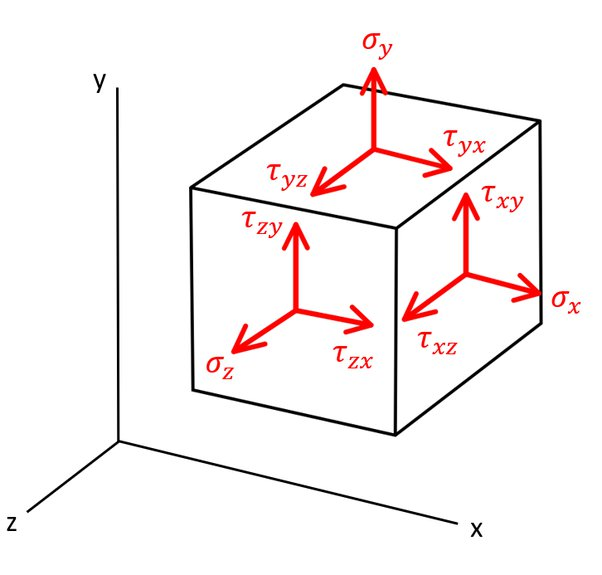
\includegraphics[width=0.1\textwidth]{shear-cube}
\end{figure}

\subsection{Newton's "law" of viscosity.}
\begin{align*}
	F/A       & = -\mu(\Delta v_x / \Delta y) = -\mu((0-v)/(y-0)) = \mu(v/y) \\
	\tau_{yx} & = -\mu(\d v_x/\d y)                                          \\
	\mu       & \equiv \ \text{viscosity of "Newtonian fluids"}              \\
	\nu       & = \ \text{Kinematic viscosity} \ \mu/\rho
\end{align*}
\begin{figure}[H]
	\centering
	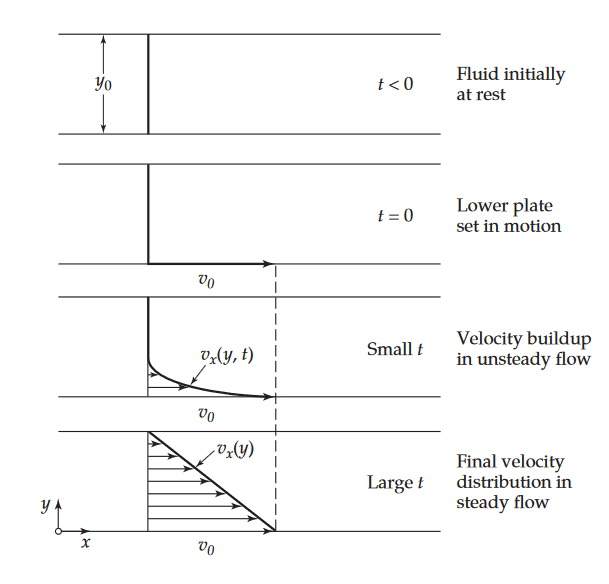
\includegraphics[width=0.25\textwidth]{newtons-law}
	\caption{BSLK Fig. 1.1-1.}
\end{figure}
Newtonian fluids are gases and simple liquids.

\subsection{Molecular origins of Newtonian viscosity.}
Consider simplest case: ideal gas, small molecules.
\begin{figure}[H]
	\centering
	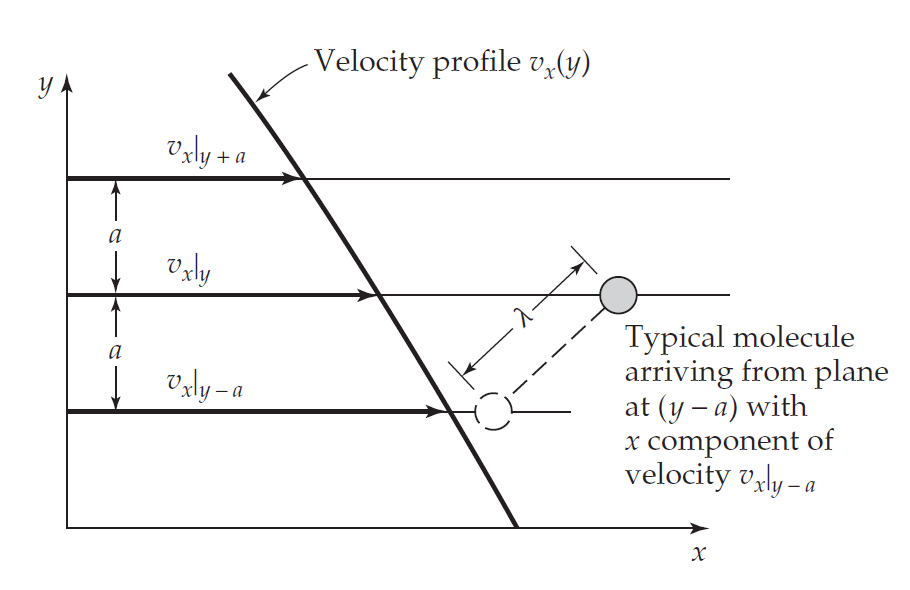
\includegraphics[width=0.2\textwidth]{molecular-origin}
	\caption{BSLK Fig. 1.6-1.}
\end{figure}
Molecules cross streamlines in random motions; they take their momentum with them when they cross.\\
Exchange of molecules between streamlines, on average, transfers momentum from fast streamlines to slow ones.\\
This momentum is transfer is the origin of "viscosity" in ideal gases (situation is more complicated in liquids).\\
In each exchange
\begin{itemize}
	\item distance is short and
	\item amount of momentum transferred is small (though there are many exchanges per unit volume per unit time)
\end{itemize}
Infinite parallel plates are impossible, so use concentric cylinders to measure viscosity.\\
If $\text{gap width}\to0$, the gap approximates planar geometry.\\
If $\text{gap width}\not\to0$, correction factors are needed.\\
This is the idea behind the Fann viscometer.

\subsection{Magnitudes of viscosity $\mu$.}
\begin{align*}
	\text{Crude oils} >> \text{Water} >> \text{Gases}
\end{align*}
Pure liquids:
\begin{itemize}
	\item $\mu$ decreases as temperature increases.
	\item $\mu$ relatively independent of pressure.
\end{itemize}
Gases at low pressures:
\begin{itemize}
	\item $\mu$ increases as temperature increases.
	\item $\mu$ independent of pressure.
\end{itemize}
Gases in or near critical region:
\begin{itemize}
	\item Trends of $\mu$ with $T$ and $P$ are complex.
\end{itemize}
Crude oils with dissolved gas:
\begin{itemize}
	\item Dissolved gas reduces $\mu$ of oil.
	\item $\mu$ decreases as $P$ decreases, until bubble point reached.
	\item $\mu$ increases as $P$ decreases further, as gas leaves solution.
\end{itemize}
\begin{figure}[H]
	\centering
	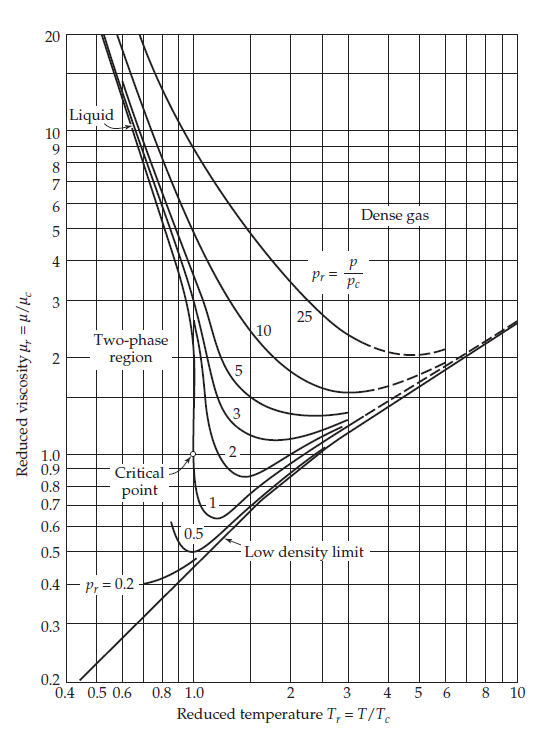
\includegraphics[width=0.15\textwidth]{reduced-viscosity}
	\caption{BSLK Fig. 1.5-1.}
\end{figure}

\subsection{Non-Newtonian fluids.}
Fluids that sometimes behave like solids: Bingham plastic.\\
Fluids that e.g. have low viscosity near well, but high viscosity away from the well: (shear-thinning) power-law fluid.\\
Recall for Newtonian fluids $\tau_{yx}=-\mu(\d v_x/\d y)$.
\begin{figure}[H]
	\centering
	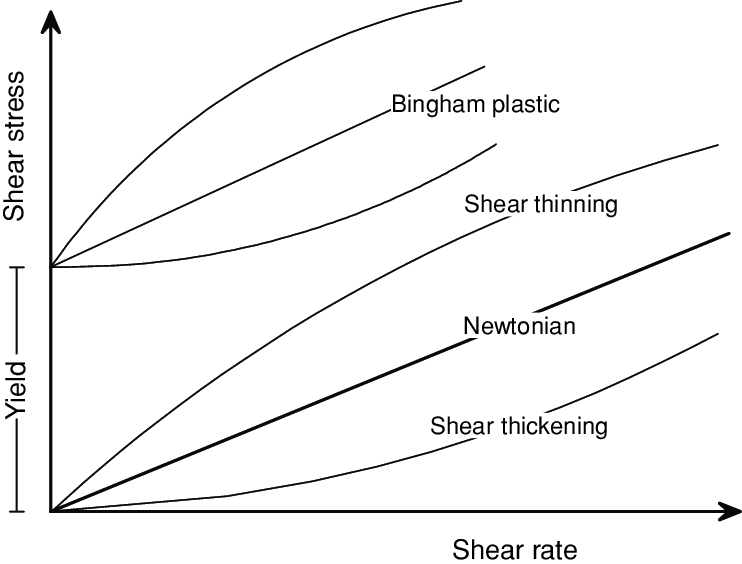
\includegraphics[width=0.2\textwidth]{fluid-types}
\end{figure}

\subsection{Bingham plastics.}
Bingham plastics are described by the following equations.
\[
	\begin{cases}
		\begin{aligned}
			\tau_{yx}           & =-\mu_0\frac{\d v_x}{\d y}+\tau_0 & \ \text{for} \ \tau_{yx}\geq\tau_0            \\
			\frac{\d v_x}{\d y} & =0                                & \ \text{for} \ -\tau_0\leq\tau_{yx}\leq\tau_0 \\
			\tau_{yx}           & =-\mu_0\frac{\d v_x}{\d y}-\tau_0 & \ \text{for} \ \tau_{yx}\geq\-\tau_0
		\end{aligned}
	\end{cases}
\]
$\mu_0$ (the slope) is sometimes called "plastic viscosity", which is not the same as (Newtonian) viscosity.\\
$\tau_0$ is the (critical) yield stress or "yield point". When $\tau_0\to0$, a Bingham plastic approaches a Newtonian fluid.

\subsection{Power-law (Ostwald-de Waele) fluids.}
Power-law fluids are described by the following equation.
\begin{align*}
	\tau_{yx}=-m\abs{\frac{\d v_x}{\d y}}^{n-1}\frac{\d v_x}{\d y}
\end{align*}
$m$ is sometimes called the "consistency index".\\
$n$ is called the "power-law index":
\begin{itemize}
	\item if $n=1$: Newtonian fluid with $m=\mu$.
	\item if $n<1$: "shear-thinning"/"pseudoplastic" where greater shear stress $\tau_{yx}\to$ much greater shear rate $\abs{\frac{\d v_x}{\d y}}$.
	\item if $n>1$: "shear-thickening/"dilatant" where greater shear stress $\tau_{yx}\to$ little increase in shear rate $\abs{\frac{\d v_x}{\d y}}$.
\end{itemize}

\section{Lecture 2.}
\subsection{Effective viscosity of non-Newtonian fluids.}
The "effective/apparent viscosity" of a non-Newtonian fluid is the viscosity of a hypothetical Newtonian fluid that would give the same result as the real fluid does in the same situation.\\
The "effective viscosity" of a non-Newtonian fluid in shear flow between parallel plates is the viscosity of a hypothetical Newtonian fluid that would give the same $\tau_{yx}$ as the real fluid does at the same $(-\d v_x/\d y)$.
\begin{figure}[H]
	\centering
	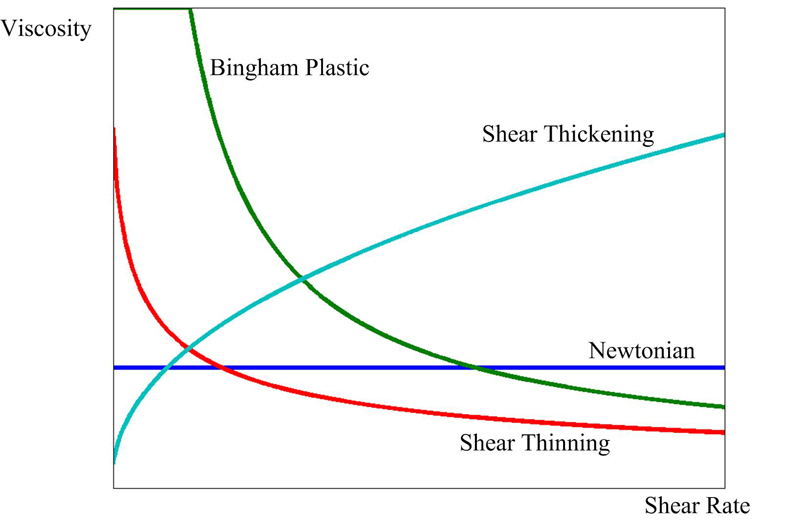
\includegraphics[width=0.25\textwidth]{viscosity-various-fluids}
\end{figure}

\subsection{Shell momentum balances.}
\begin{align*}
	\begin{pmatrix}\text{rate of momentum} \\ \text{in by convection}\end{pmatrix}
	 & -\begin{pmatrix}\text{rate of momentum} \\ \text{out by convection}\end{pmatrix}                \\
	+\begin{pmatrix}\text{rate of momentum} \\ \text{in by shear force}\end{pmatrix}
	 & -\begin{pmatrix}\text{rate of momentum} \\ \text{out by shear force}\end{pmatrix}               \\
	+\begin{pmatrix}\text{body forces (gravity)} \\ \text{acting on fluid}\end{pmatrix}
	 & =\begin{pmatrix}\text{accumulation of} \\ \text{momentum} \\ \text{(acceleration)}\end{pmatrix}
\end{align*}
First four terms: momentum crossing boundaries.\\
Last two terms: within system volume (boundaries).\\
Accumulation of momentum is zero at steady state.

\subsection{Shell momentum balance procedure.}
\textit{BSLK §2.1.}
\begin{enumerate}
	\item Select coordinate system, define control volume (boundaries either $\parallel$ or $\bot$ to velocity and thin in any direction in which velocity varies).
	\item State boundary conditions.*
	\item Perform momentum balance.**
	\item Thickness $\to0$ (gives differential equation for $\tau$).
	      \begin{enumerate}
		      \item (optional) solve differential equation for $\tau$, apply boundary condition if boundary condition applies to $\tau$ alone.
	      \end{enumerate}
	\item Relate $\tau$ to $\d v/\d x$ (apply constitutive equation).
	\item Solve differential equation for $v$, apply boundary conditions.
\end{enumerate}
*\textbf{Boundary conditions}:
\begin{enumerate}
	\item Specify $v$ at solid surface.
	      \begin{enumerate}
		      \item fluid $v$ is equal to solid velocity at solid wall.
	      \end{enumerate}
	\item Specify $\tau$ at fluid surface.
	      \begin{enumerate}
		      \item in liquid, $\tau=0$ at gas interface.
		      \item $\tau$, $v$ continuous across liquid-liquid interface.
	      \end{enumerate}
	\item $\tau$, $v$ not infinite anywhere in region of interest.
\end{enumerate}
**\textbf{Elements of momentum balance}:\\
Momentum flux ($\propto$ area), called "$\phi$" tensor.
\begin{enumerate}
	\item Convection of momentum through surface.
	\item Shear stress $\tau$ on surface ("molecular transport of momentum").
	\item Pressure pressing inward on surface.
\end{enumerate}
Momentum "generation" or "source" ($\propto$ volume).
\begin{enumerate}
	\setcounter{enumi}{3}
	\item Body forces within volume.
\end{enumerate}
Momentum accumulation ($\propto$ volume) (not a steady state!).
\begin{enumerate}
	\setcounter{enumi}{4}
	\item Acceleration of system mass - $\p(\rho v)/\p t$.
\end{enumerate}

\subsection{Four aspects can vary from one problem to another.}
\begin{itemize}
	\item Geometry (coordinate system).
	\item Elements in momentum balance.
	\item Constitutive equation (relation between $\tau$ and $\frac{\d v_x}{\d y}$).
	\item Boundary conditions.
\end{itemize}

\section{Lecture 3.}
		\section{Lecture notes}
Definition of $\Delta\mathscr{P}$
\[
	\Delta\mathscr{P}\equiv(p_0-p_L)+\rho g[(\text{vertical position}_0-(\text{vertical position}_L))]\tag{Lecture notes 3.17}
\]
Assumptions behind derivations in Chapter 2 (Re!)
\[
	\textit{see lecture notes}\tag{Lecture notes 3.22}
\]
\section{Chapter 1: Viscosity and the Mechanisms of Momentum Transport}
Newton's law of viscosity
\[
	\tau_{yz}=-\mu\frac{\d v_x}{\d y}\tag{1.2-2}
\]
Bingham plastic
\[
	\begin{cases}
		\begin{aligned}
			\tau_{yx}           & =-\mu_0\frac{\d v_x}{\d y}+\tau_0 & \tau_{yx}\geq\tau_0            \\
			\frac{\d v_x}{\d y} & =0                                & -\tau_0\leq\tau_{yx}\leq\tau_0 \\
			\tau_{yx}           & =-\mu_0\frac{\d v_x}{\d y}-\tau_0 & \tau_{yx}\geq\-\tau_0
		\end{aligned}
	\end{cases}\tag{Lecture notes 2.6}
\]
Power-law fluid
\begin{align*}
	\tau_{yx}=-m\abs{\frac{\d v_x}{\d y}}^{n-1}\frac{\d v_x}{\d y}\tag{Lecture notes 2.8}
\end{align*}
Kinematic viscosity
\[
	\nu = \mu/\rho\tag{1.2-3}
\]
\section{Chapter 2: Shell Momentum Balances and Velocity Distributions in Laminar Flow}
\subsection{\S2.2 Flow of a Falling Film (BSL1)}
Momentum balance
\[
	LW\tau_{xz|x}-LW\tau_{xz|x+\Delta x}+LW\Delta x\rho g\cos\beta=0\tag{2.2-6}
\]
%\[
%	\lim_{\Delta x\to0}\left(\frac{\tau_{xz|x+\Delta x}-\tau_{xz|x}}{\Delta x}\right) = \rho g\cos\beta\tag{2.2-7}
%\]
%\[
%	\tau_{xz}=\rho gx\cos\beta+C_1\tag{2.2-9}
%\]
Momentum flux distribution% with $\tau_{xz}=0$ at $x=0$
\[
	\tau_{xz}=\rho gx\cos\beta+C_1\tag{2.2-9}
\]
Velocity distribution% with $v_z=0$ at $x=\delta$
\[
	v_z=\frac{\rho g\delta^2\cos\beta}{2\mu}\left[1-\left(\frac{x}{\delta}\right)^2\right]\tag{2.2-16}
\]
Maximum velocity
\[
	v_{z,\text{max}}=\frac{\rho g\delta^2\cos\beta}{2\mu}\tag{2.2-17}
\]
Average velocity
\[
	\langle v_z\rangle=\frac{\rho g\delta^2\cos\beta}{3\mu}\tag{2.2-18}
\]
Volume flow rate
\[
	Q=\frac{\rho gW\delta^3\cos\beta}{3\mu}\tag{2.2-19}
\]
Film thickness
\[
	\delta=\sqrt[3]{\frac{3\mu\Gamma}{\rho^2 g\cos\beta}}\tag{2.2-20}
\]
Force of the fluid on the surface
\[
	F_z=\rho g\delta LW\cos\beta\tag{2.2-21}
\]
Momentum flux distribution with variable viscosity
\[
	\tau_{xz}=-\mu_0e^{-\alpha(x/\delta)}\frac{\d v_z}{\d x}=\rho gx\cos\beta\tag{2.2-23}
\]
Velocity distribution with variable viscosity
\[
	v_z=\frac{\rho g\delta^2\cos\beta}{\mu_0}\left[e^\alpha\left(\frac{1}{\alpha}-\frac{1}{\alpha^2}\right)-e^{\alpha x/\delta}\left(\frac{x}{\alpha\delta}-\frac{1}{\alpha^2}\right)\right]\tag{2.2-24}
\]
Average velocity with variable viscosity
\[
	\langle v_z\rangle=\frac{\rho g\delta^2\cos\beta}{\mu_0}\left[e^\alpha\left(\frac{1}{\alpha}-\frac{2}{\alpha^2}+\frac{2}{\alpha^3}\right)-\frac{2}{\alpha^3}\right]\tag{2.2-26}
\]
\subsection{\S2.3 Flow Through a Circular Tube (BSL1)}
Momentum balance
\[
	\textit{see text}\tag{2.3-8}
\]
Momentum flux distribution
\[
	\tau_{rz}=\left(\frac{\mathscr{P}_0-\mathscr{P}_L}{2L}\right)r+\frac{C_1}{r}\tag{2.3-11}
\]
Velocity distribution
\[
	v_z=\frac{(\mathscr{P}_0-\mathscr{P}_L)R^2}{4\mu L}\left[1-\left(\frac{r}{R}\right)^2\right]\tag{2.3-16}
\]
Maximum velocity
\[
	v_{z,\text{max}}=\frac{(\mathscr{P}_0-\mathscr{P}_L)R^2}{4\mu L}\tag{2.3-17}
\]
Average velocity
\[
	\langle v_z\rangle=\frac{(\mathscr{P}_0-\mathscr{P}_L)R^2}{8\mu L}\tag{2.3-18}
\]
Volume flow rate
\[
	Q=W/\rho=\frac{\pi(\mathscr{P}_0-\mathscr{P}_L)R^4}{8\mu L}\tag{2.3-19}
\]
Force of the fluid on the surface
\[
	F_z=\pi R^2(p_0-p_L)+\pi R^2L\rho g\tag{2.3-20}
\]
Velocity distribution for Bingham flow
\[
	v_z^>=\frac{(\mathscr{P}_0-\mathscr{P}_L)R^2}{4\mu_0 L}\left[1-\left(\frac{r}{R}\right)^2\right]-\frac{\tau_0 R}{\mu_0}\left[1-\left(\frac{r}{R}\right)\right] \quad r\geq r_0\tag{2.3-25}
\]
\[
	v_z^<=\frac{(\mathscr{P}_0-\mathscr{P}_L)R^2}{4\mu_0 L}\left(1-\frac{r_0}{R}\right)^2\quad r\leq r_0\tag{2.3-26}
\]
Volume flow rate for Bingham flow
\[
	\textit{see text}\tag{2.3-30}
\]
Equations for power-law fluids in Lecture notes 3.6.\\
Effective viscosity for tube flow
\[
	\mu_{\text{eff}}=\frac{\pi R^4\Delta\mathscr{P}}{8LQ}\tag{Lecture notes 3.8}
\]
\subsection{\S2.4 Flow Through an Annulus (BSL1)}
\textit{Same momentum balance as Circular Tube}\\
Momentum flux distribution
\[
	\tau_{rz}=\frac{(\mathscr{P}_0-\mathscr{P}_L)R}{2L}\left[\left(\frac{r}{R}\right)-\left(\frac{1-\kappa^2}{2\ln(1/\kappa)}\right)\left(\frac{R}{r}\right)\right]\tag{2.4-12}
\]
Velocity distribution
\[
	v_z=\frac{(\mathscr{P}_0-\mathscr{P}_L)R^2}{4\mu L}\left[1-\left(\frac{r}{R}\right)^2+\left(\frac{1-\kappa^2}{\ln(1/\kappa)}\right)\ln\left(\frac{r}{R}\right)\right]\tag{2.4-13}
\]
\textit{See text for more quantities}\\
Equations for Bingham plastics and Power-law liquids in Lecture notes 3.13.
\subsection{\S2.7 Flow Around a Sphere}
Viscosity of fluid from terminal velocity of falling sphere
\[
	\mu=\frac{2}{9}\frac{R^2(\rho_s-\rho)g}{v_t}\tag{2.7-17}
\]
Suspension of particles in Bingham plastic
\[
	\tau_0\geq\frac{4}{3\pi}R\left|\rho_s-\rho\right|g\tag{Lecture notes 3.21}
\]
\subsection{2B.4 Laminar Flow in a Narrow Slit}
Momentum-flux distribution
\[
	\tau_{xz}(x)=\left(\frac{\mathscr{P}_0-\mathscr{P}_L}{L}\right)x\tag{2B.4-1}
\]
Velocity distribution
\[
	v_z(x)=\frac{(\mathscr{P}_0-\mathscr{P}_L)B^2}{2\mu L}\left[1-\left(\frac{x}{B}\right)^2\right]\tag{2B.4-2}
\]
Volume flow rate
\[
	Q=\frac{2}{3}\frac{(\mathscr{P}_0-\mathscr{P}_L)B^3W}{\mu L}
\]
Equations for Bingham plastics in Lecture notes 3.10.\\
Equations for Power-law liquids in Lecture notes 3.12.
\section{Chapter 6: Interphase Transport in Isothermal Systems}
\subsection{\S6.1 Definition of Friction Factors}
General definition of friction factor
\[
	F_k=AKf\tag{6.1-1}
\]
\subsection{\S6.2 Friction Factors for Flow in Tubes}
$F_k$ for flow in conduits
\[
	F_k=(2\pi RL)\left(\frac{1}{2}\rho\langle\overline{v}_z\rangle^2\right)f\tag{6.1-2}
\]
$f$ for flow in conduits
\[
	f=\frac{1}{4}\left(\frac{D}{L}\right)\left(\frac{\mathscr{P}_0-\mathscr{P}_L}{\frac{1}{2}\rho\langle\overline{v}_z\rangle^2}\right)\tag{6.1-4}
\]
Correlations for $f$
\[
	f(\text{Re})=\frac{16}{\text{Re}}\left\{\begin{aligned}&\text{Re}<2100 \ \text{stable}\\&\text{Re}>2100 \ \text{usually unstable}\end{aligned}\right\}\tag{6.2-11}
\]
Friction factor for tube flow
\[
	\textit{see figure}\tag*{\textbf{Fig. 6.2-2}}
\]
Friction factor for turbulent flow in non-circular tubes
\[
	f=\left(\frac{R_h}{L}\right)\left(\frac{\mathscr{P}_0-\mathscr{P}_L}{\frac{1}{2}\rho\langle\overline{v}_z\rangle^2}\right)\tag{6.2-16}
\]
Mean hydraulic radius for rectangular slit
\[
	R_h=B\tag{Lecture notes 9.6}
\]
\subsection{\S6.3 Friction Factors for Flow Around Spheres}
$F_k$ for flow around submerged objects
\[
	F_k=(\pi R^2)\left(\frac{1}{2}\rho v_\infty^2\right)f\tag{6.1-5}
\]
$f$ for flow around submerged objects
\[
	f=\frac{4}{3}\frac{gD}{v_\infty^2}\left(\frac{\rho_\text{sph}-\rho}{\rho}\right)\tag{6.1-7}
\]
Re for flow around spheres
\[
	\text{Re}\equiv\frac{Dv_\infty\rho}{\mu}=\frac{2Rv_\infty\rho}{\mu}\tag{6.3-8}
\]
$F_k$ for flow around spheres
\[
	F_k=(\pi R^2)\left(\frac{1}{2}\rho v_\infty^2\right)\left(\frac{24}{Dv_\infty\rho/\mu}\right)\tag{6.3-14}
\]
Correlation for $f$
\begin{align}
	f & \approx\frac{24}{\text{Re}} \                               & \text{for Re}\leq0.1\tag{6.3-15}              \\
	f & \approx\left(\sqrt{\frac{24}{\text{Re}}}+0.5407\right)^2 \  & \text{for Re}\leq6000\tag{6.3-16}             \\
	f & \approx0.44 \                                               & \text{for} \ 500<\text{Re}<100000\tag{6.3-17}
\end{align}
Friction factor for spheres moving relative to fluid
\[
	\textit{see figure}\tag*{\textbf{Fig. 6.3-1}}
\]
\subsection{\S6.4 Friction Factors for Packed Columns}
Re for packed columns
\[
	\text{Re}=\frac{D_pv_0\rho}{\mu}\left(\frac{1}{1-\varepsilon}\right)\tag{Lecture notes 9.20}
\]
Blake-Kozeny equation
\[
	\frac{\mathscr{P}_0-\mathscr{P}_L}{L}=150\left(\frac{\mu v_0}{D_p^2}\right)\frac{(1-\varepsilon)^2}{\varepsilon^3}\tag{6.4-9}
\]
Correlation for $f$
\[
	\textit{see figure}\tag*{\textbf{Fig. 6.4-2}}
\]
\textit{More in lecture notes and \S6.4}
\section{Chapter 7: Macroscopic Balances for Isothermal Flow Systems}
\subsection{\S7.5 Estimation of the Viscous Loss}
Macroscopic mechanical energy balance
\[
	\frac{1}{2}(v_2^2-v_1^2)+g(h_2-h_1)+\int_{p_1}^{p_2}{\frac{1}{\rho}\d p}=\hat{W}_m-\hat{E}_v\tag{7.5-11}
\]
For turbulent flow in tubes of circular cross section
\[
	\textit{see text}\tag{7.5-12}
\]
Brief summary of friction-loss factors
\[
	\textit{see table}\tag*{\textbf{Table 7.5-1}}
\]
\section{Examples in Lecture Notes}
\[
	\text{Determination of Viscosity from Capillary Flow Data}\tag{BSL1 2.3-1}
\]
\[
	\text{Given $\Delta\mathscr{P}/L$, compute $Q$}\tag{Lecture notes 9.9}
\]
\[
	\text{Examples of trial-and-error method}\tag{Lecture notes 9.11}
\]
\[
	\text{Solving for unknown Re}\tag{Lecture notes 9.15}
\]
%		\newpage
		\section{Chapter 9: Thermal Conductivity and the Mechanisms of Energy Transport}
\subsection{\S9.2 Conductive Heat-Flux Vector --- Fourier's Law}
Fourier's law of heat conduction (in one dimension)
\[
	\left(\frac{Q}{A}=\right)q_y=-k\frac{\d T}{\d y}\tag{9.2-2}
\]
Conductive heat-flow vector
\[
	\vec{q}=-k\grad{T}\tag{9.2-6}
\]
Thermal diffusivity
\[
	\alpha=\frac{k}{\rho\hat{C}_p}\tag{9.2-7}
\]
Prandtl number
\[
	\text{Pr} = \frac{\nu}{\alpha}=\frac{\hat{C}_p\mu}{k}\tag{9.2-8}
\]
Development of steady-state temperature profile between plates
\[
	\textit{see figure}\tag*{\textbf{Fig. 9.2-1}}
\]
Summary of units
\[
	\textit{see table}\tag*{\textbf{Table 9.2-1}}
\]
\subsection{\S9.5 Thermal Conductivity Data from Experiments}
References for values of $k$, $\hat{C}_p$, and $\text{Pr}$
\[
	\textit{see table}\tag*{\textbf{Tables 9.5-1 to 9.5-3}}
\]
\section{Chapter 10: Shell Energy Balances and Temperature Distributions in Solids and Laminar Flow}
\subsection{BSL1 \S9.1 Shell Energy Balances: Boundary Conditions}
Steady-state shell energy balance
\[
	\textit{see text}\tag{9.1-1}
\]
Outline of shell energy balance approach
\[
	\textit{see lecture notes}\tag*{Lecture notes 11.3}
\]
Newton's law of cooling
\[
	q=h(T-T_\text{fluid})\tag{9.1-2}
\]
Preview of BSL1 chapter 9
\[
	\textit{see table}\tag*{Lecture notes 11.4}
\]
\subsection{BSL1 \S9.2 Heat Conduction with an Electrical Heat Source}
Rate of heat production per unit volume
\[
	S_e=\frac{I^2}{k_e}\tag{9.2-1}
\]
Heat-flux distribution
\[
	q_r=\frac{S_er}{2}\tag{9.2-9}
\]
Temperature rise as a parabolic function of $r$
\[
	T(r)-T_0=\frac{S_eR^2}{4k}\left[1-\left(\frac{r}{R}\right)^2\right]\tag{9.2-13}
\]
Maximum temperature rise (at $r=0$)
\[
	T_\text{max}-T_0=\frac{S_eR^2}{4k}\tag{9.2-14}
\]
Average temperature rise
\[
	\langle T\rangle-T_0=\frac{S_eR^2}{8k}\tag{9.2-15}
\]
Heat flow at the surface
\[
	Q|_{r=R}=\pi R^2L\cdot S_e\tag{9.2-16}
\]
\subsection{BSL1 \S9.3 Heat Conduction with a Nuclear Heat Source}
Volume source of thermal energy
\[
	S_n=S_{n0}\left[1+b\left(\frac{r}{R^{(F)}}\right)^2\right]\tag{9.3-1}
\]
Heat-flux distribution in the fissionable sphere
\[
	q_r^{(F)}=S_{n0}\left(\frac{r}{3}+\frac{b}{R^{(F)2}}\frac{r^3}{5}\right)\tag{9.3-12}
\]
Heat-flux distribution in the spherical shell cladding
\[
	q_r^{(C)}=S_{n0}R^{(F)3}\left(\frac{1}{3}+\frac{b}{5}\right)\frac{1}{r^2}\tag{9.3-13}
\]
Temperature profiles
\[
	T^{(F)}-T_0=\textit{see text}\tag{9.3-20}
\]
\[
	T^{(C)}-T_0=\frac{S_{n0}R^{(F)2}}{3k^{(C)}}\left(1+\frac{3}{5}b\right)\left(\frac{R^{(F)}}{r}-\frac{R^{(F)}}{R^{(C)}}\right)\tag{9.3-21}
\]
\subsection{BSL1 \S9.4 Heat Conduction with a Viscous Heat Source}
Volume source of thermal energy
\[
	S_v=-\tau_{xz}\left(\frac{\d v_z}{\d x}\right)=\mu\left(\frac{\d v_z}{\d x}\right)^2\tag{9.4-1}
\]
\subsection{BSL1 \S9.5 Heat Conduction with Chemical Heat Source}
Volume rate of thermal energy production by chemical reactions
\[
	S_c=S_{c1}\left(\frac{T-T^\circ}{T_1-T^\circ}\right)\tag{9.5-1}
\]
\subsection{BSL1 \S9.6 Heat Conduction Through Composite Walls: Addition of Resistances}
Heat-flux distribution
\[
	q_0=\frac{T_a-T_b}{\left(\frac{1}{h_0}+\sum_{i=1}^{3}\frac{x_i-x_{i-1}}{k^{i-1,i}}+\frac{1}{h_3}\right)}\tag{9.6-15}
\]
Heat-flux distribution, rewritten
\[
	q_0 = U(T_a-T_0) \quad \text{or} \quad Q_0=U(WH)(T_a-T_b)\tag{9.6-16}
\]
Over-all heat transfer coefficient
\[
	U=\left(\frac{1}{h_0}+\sum_{i=1}^{3}\frac{x_i-x_{i-1}}{k^{i-1,i}}+\frac{1}{h_3}\right)^{-1}\tag{9.6-17}
\]
Composite cylindrical walls (Lecture notes 15.6)
\[
	Q_0 = 2\pi Lr_0q_0 =...\tag{9.6-29}
\]
\[
	Q_0=U_0(2\pi r_0L)(T_a-T_b)\tag{9.6-30}
\]
\[
	U_0=r_0^{-1}\left(\frac{1}{r_0h_0}+\sum_{i=1}^{3}\frac{\ln r_r/r_{i-1}}{k^{i-1,i}}+\frac{1}{r_3h_3}\right)^{-1}\tag{9.6-31}
\]
\subsection{BSL1 \S9.7 Heat Conduction in a Cooling Fin}
%Dimensionless temperature
%\[
%	\Theta=\frac{T-T_a}{T_w-T_a}\tag{9.7-6}
%\]
%Dimensionless distance
%\[
%	\zeta=\frac{z}{L}\tag{9.7-7}
%\]
%Dimensionless heat transfer coefficient
%\[
%	N=\sqrt{\frac{hL^2}{kB}}\tag{9.7-8}
%\]
Dimensionless temperature, rewritten
\[
	\Theta=\frac{\cosh N(1-\zeta)}{\cosh N}\tag{9.7-13}
\]
\subsection{BSL1 \S9.8 Forced Convection}
Velocity profile
\[
	v_z=v_{z,\text{max}}\left[1-\left(\frac{r}{R}\right)^2\right]\tag{9.8-1}
\]
%Conduction
%\[
%	q_r=-k\frac{\p T}{\p r} \qquad q_z=-k\frac{\p T}{\p z}\tag{9.8-10}
%\]
Partial differential equation
\[
	\rho\hat{C}_pv_\text{max}\left[1-\left(\frac{r}{R}\right)^2\right]\frac{\p T}{\p z} = k\frac{1}{r}\frac{\p}{\p r}\left(r\frac{\p T}{\p r}\right)\tag{9.8-12}
\]
\section{Chapter 11: The Equations of Change for Nonisothermal Systems}
\subsection{\S11.5 The Equations of Change and Solving Problems with Two Independent Variables}
Velocity distribution in dimensionless form for flow in the neighbourhood of a wall suddenly set in motion
\[
	\textit{see figure}\tag*{\textbf{Fig. 3.8-2} (b)}
\]
Temperature difference
\[
	\frac{T(y,t)-T_0}{T_1-T_0}=1-\erf\frac{y}{\sqrt{4\alpha t}}\tag{11.5-10}
\]
Wall heat flux
\[
	q_y|_{y=0}=-k\frac{\p T}{\p y}\bigg|_{y=0}=\frac{k}{\sqrt{\pi\alpha t}}(T_1-T_0)\tag{11.5-12}
\]
Initial condition
\[
	\text{at} \ t\leq0, \ T=T_0 \ \text{for all} \ y\tag{11.5-2}
\]
Temperature profiles for unsteady-state heat conduction in a slab of finite thickness $2b$
\[
	\textit{see figure}\tag*{\textbf{Fig. 11.5-1}}
\]
Temperature profiles for unsteady-state heat conduction in a cylinder of radius $R$
\[
	\textit{see figure}\tag*{\textbf{Fig. 11.5-2}}
\]
Temperature profiles for unsteady-state heat conduction in a sphere of radius $R$.
\[
	\textit{see figure}\tag*{\textbf{Fig. 11.5-3}}
\]
\section{Chapter 14: Interphase Transport in Nonisothermal Systems}
\subsection{\S14.1 Definitions of Heat-Transfer Coefficients}
Heat-transfer coefficient
\[
	Q=hA\Delta T\tag{14.1-1}
\]
Heat-transfer coefficients for the fluid in the heated section (Eq. I)
%\[
%	Q=h_1(\pi DL)(T_{01}-T_{b1})\equiv h_1(\pi DL)\Delta T_1\tag{14.1-2}
%\]
\begin{align*}
	Q & =h_{\ln}(\pi DL)\left(\frac{(T_{01}-T_{b1})-(T_{02}-T_{b2})}{\ln(T_{01}-T_{b1})-\ln(T_{02}-T_{b2})}\right) \\
	  & \equiv h_{\ln}(\pi DL)\Delta T_{\ln}\tag{14.1-4}
\end{align*}
Energy balance in tube (Eq. II)
\[
	w\hat{C}_pT_{b1} - w\hat{C}_pT_{b2} + Q=0 \quad \text{or} \quad Q=w\hat{C}_p(T_{b2}-T_{b1})\tag{14.1-10}
\]
Definition of $h_{\ln}$
\[
	h_{\ln}=\frac{w\hat{C}{p}}{\pi D^2}\frac{(T_{b2}-T_{b1})}{(T_0-T_b)_{\ln}}\left(\frac{D}{L}\right)\tag{14.1-14}
\]
Heat balance with definition of $h_{\ln}$ (Eq. III)
\[
	\frac{h_{\ln}D}{k} \equiv \text{Nu}_{\ln}=\frac{(T_{b2}-T_{b1})}{(T_0-T_b)_{\ln}}\left(\text{Re}\text{Pr}\frac{D}{4L}\right)\tag*{Lecture notes 15.2}
\]
For uniform $T_0$ along tube ($T_{01}=T_{02}\equiv T_0$) (ALWAYS assumed!)
\[
	\frac{(T_{b2}-T_{b1})}{(T_0-T_b)_{\ln}}=\ln\left(\frac{T_0-T_{b1}}{T_0-T_{b2}}\right)=\ln\frac{\Delta T \ \text{at inlet}}{\Delta T \ \text{at outlet}}\tag*{Lecture notes 15.2}
\]
Heat transfer in a circular tube
\[
	\textit{see figure}\tag*{\textbf{Fig. 14.1-1}}
\]
\subsection{\S14.2 Heat-Transfer Coefficients For Forced Convection Through Tubes and Slits Obtained From Solutions of the Equations of Change}
Nusselt number for fully developed, laminar flow of Newtonian fluids with constant physical properties
\[
	\textit{see figure}\tag*{\textbf{Fig. 14.2-1}}
\]
\subsection{\S14.3 Empirical Correlations for Heat-Transfer Coefficients for Forced Convection in Tubes}
Nusselt number
\[
	\text{Nu}_{\ln}\equiv\frac{h_{\ln}D}{k}\tag*{Lecture notes 15.4}
\]
Reynolds number
\[
	\text{Re}\equiv\frac{Dv\rho}{\mu}=\frac{DG}{\mu}\tag*{Lecture notes 15.4}
\]
Prandtl number
\[
	\text{Pr}\equiv\frac{\hat{C}_p\mu}{k}\tag*{Lecture notes 15.4}
\]
Nusselt number for highly turbulent flow
\[
	\text{Nu}_{\ln}=0.026\ \text{Re}^{0.8}\text{Pr}^{1/3}\left(\frac{\mu_b}{\mu_0}\right)^{0.14}\tag{14.3-16}
\]
Nusselt number for laminar flow
\[
	\text{Nu}_{\ln}=1.86\left(\text{Re}\text{Pr}\frac{D}{L}\right)^{1/3}\left(\frac{\mu_b}{\mu_0}\right)^{0.14}\tag{14.3-17}
\]
Mean hydraulic radius for non-circular tubes
\[
	4R_h=4(S/Z)=D\tag*{Lecture notes 15.5}
\]
Conservation equation (modified form of Eq. III)
\[
	\left[\frac{U_0D_0}{k}\right]=\ln\left(\frac{T_f-T_{b1}}{T_f-T_{b2}}\right)\text{Re}\text{Pr}\frac{D_0}{4L}\tag*{Lecture notes 15.6}
\]
Heat-transfer coefficients for fully developed flow in smooth tubes
\[
	\textit{see figure}\tag*{\textbf{Fig. 14.3-2}}
\]
%\section{Chapter 17: Diffusivity and the Mechanisms of Mass Transport}
\section{Mass Transfer}
Diffusivity
\[
	\mathscr{D}_{AB}\tag*{Lecture notes 19.1}
\]
Molar flux
\[
	N_A=\frac{\mathscr{D}}{\sqrt{\pi \mathscr{D}t}}(c_{s1}-c_{s0})\tag*{Lecture notes 19.3}
\]
\subsection{Mass transfer in tubes}
Definition of mass-transfer coefficient (Eq. Im)
\[
	\mathscr{W}_A^{(m)}=k_{x,\ln}(\pi DL)(x_{A0}-x_{Ab})_{\ln}\tag*{Lecture notes 20.1}
\]
Mass-conservation equation (Eq. IIm)
\[
	\mathscr{W}_A^{(m)}=(c_{AB2}-c_{AB1})\pi R^2\langle v\rangle\tag*{Lecture notes 20.1}
\]
(Eq IIIm)
\[
	\frac{k_{x,\ln}D}{c\mathscr{D}_{AB}}=\text{Sh}=\ln\left[\frac{c_{A0}-c_{AB1}}{c_{A0}-c_{AB2}}\right]\text{Re}\text{Sc}\frac{D}{4L}\tag*{Lecture notes 20.1}
\]
Correlations
\[
	\textit{see notes}\tag*{Lecture notes 20.3}
\]
		
		\newpage
	\end{multicols}
\end{document}













